%%%%%%%%%%%%%%%%%%%%%%%%%%%%%%%%%%%%%%%%%%%%%%%%%%%%%%%%%%%%%%%%%%%%%%%%%%%%%%%%
%2345678901234567890123456789012345678901234567890123456789012345678901234567890
%        1         2         3         4         5         6         7         8

\documentclass[letterpaper, 10 pt, conference]{ieeeconf}  % Comment this line out if you need a4paper

%\documentclass[a4paper, 10pt, conference]{ieeeconf}      % Use this line for a4 paper

\IEEEoverridecommandlockouts                              % This command is only needed if 
                                                          % you want to use the \thanks command

\overrideIEEEmargins                                      % Needed to meet printer requirements.

% See the \addtolength command later in the file to balance the column lengths
% on the last page of the document

% The following packages can be found on http:\\www.ctan.org
\usepackage{graphics} % for pdf, bitmapped graphics files
\usepackage{epsfig} % for postscript graphics files
\usepackage{mathptmx} % assumes new font selection scheme installed
\usepackage{times} % assumes new font selection scheme installed
\usepackage{amsmath} % assumes amsmath package installed
\usepackage{amssymb}  % assumes amsmath package installed
\usepackage{hyperref}
%\usepackage{algorithm}
%\usepackage{algpseudocode}
\usepackage{blindtext}
\usepackage{subcaption}
\usepackage{graphicx}
\usepackage{balance}
\usepackage[ruled,vlined,linesnumbered]{algorithm2e}

\title{\LARGE \bf
Report of Applying ADMM to Neural Network
}


\author{Qunjie Zhou and Zhenzhang Ye% <-this % stops a space
}

\begin{document}

\maketitle
\thispagestyle{empty}
\pagestyle{empty}

%%%%%%%%%%%%%%%%%%%%%%%%%%%%%%%%%%%%%%%%%%%%%%%%%%%%%%%%%%%%%%%%%%%%%%%%%%%%
\section{INTRODUCTION}
\subsection{Artificial Neural Networks} 
Artificial neural networks(ANN) are computational models, inspired by natural neural networks to learn useful information(representation) from data. They have been widely applied to tackle real-world problems and brought breakthrough to fields such as image recognition and natural language processing.  Before a neural network can actually perform pattern recognition tasks, it requires numerous learning on a specific dataset, which refers to the training process.
 
 In ANN, a neuron as the core composing unit can be mathematically represented as a function $g: a \rightarrow z$
 \begin{equation}
	g(a, W)= h(\displaystyle\sum_{k}a_kw_k) = h(Wa)
\end{equation}
where $a$ is the input data, $W$ is the weight matrix (Here we consider bias is integrated into $W$) and $h$ is an activation function\cite{1}. A layer is composed by a set of artificial neurons with identical activation function. A feed-forward neural network where the output of neurons of previous layer is feed forward to the neurons of current layer, can be formed by consecutively connecting multiple layers.

To be specific, a 3-layer feed-forward neural network can be mathematical defined as:
\begin{equation} \label{eq:network}
	f(a_0, W) = W_3(h_2(W_2(h_1(W_1a_0))))
\end{equation}
where $W = \{W_1, W_2, W_3\}$ denotes the ensemble of weight ma- trices, and each column of input $a_0$ is a training sample.

\subsection{Training a neural network with SGD }
Such a neural network defined in (\ref{eq:network}) is learned by varying weight matrix $W$ so that the output activation $a_L$ match to the target label $y$. Using a loss function $l$ as the evaluation criteria, the training task can be proposed as an optimization problem:
\begin{equation} \label{eq:min}
	\min_{W} l(f(a_0, W), y)
\end{equation}
As the activation function $h$ introduces non-linearity into the network model, problem (\ref{eq:min}) results in a highly non-convex optimisation problem. The most extensively applied approach for training a neural network is stochastic gradient descent (SGD), using backpropagation to calculate the gradients.  Although SGD performs well in serial setting where modern GPUs are necessary for efficient training, it fails to maintain strong scaling when parallelizing over CPUs machines \cite{2}. In addition, the class of gradient descent based approaches also has the severe problem of being trapped in poor local optima \cite{3} or a saddle point \cite{4}, especially for deeper architecture. 

\subsection{Alternating Direction Method of Multipliers}
In the context of optimisation, except for the gradient-based algorithms, there are still more sophisticated optimisation methods. The alternating direction method with multipliers (ADMM) has been one of most powerful and successful methods for solving constrained convex problems. Recent studies (e.g. \cite{5, 6, 7, 8}) on ADMM for non-convex optimization problem, show that ADMM also performs well on a broad class of solve non-convex problems. Compared with SGD methods, in ADMM the original complex problem is decomposed into several simpler subproblems that are often solvable in closed form. Furthermore, the decomposition leads to possibility of large-scale distributed computing environments.

In this project, we are interested applying a specific optimisation method ADMM to the training task. We follow the approach proposed in work \cite{9} and investigate whether ADMM can get rid of the troubles of SGD mentioned before.  In section \ref{preliminaries}, we state the concrete problem with mathematic notations. The Goldstein ADMM method proposed by work \cite{9} is fully studied in section \ref{studycase}, with practical experiments and theoretical analysis. In the following section \ref{improvement}, an improved version of this method is proposed and demonstrated. Then, the section \ref{experiment}, the improved version is extensively evaluated on different datasets and compared with various optimization approaches. Finally, section \ref{conclusion} comes to a conclusion based on previous results.

\section{Preliminaries}\label{preliminaries}
To verify the feasibility of training ANN with ADMM, we select the simplest feed-forward neural network as our training model. To define the problem, let's assume the network consists of $L$ layers. Given an input $a_{l-1}$ and its label $y$, the goal of training is to find the best weight $W$ which minimizes a loss function $\mathcal{L}$. The concrete mathematical model is defined as: 
\begin{equation}
\begin{aligned} 
& \underset{\{W_l\},\{a_l\}, \{z_l\}}{\text{minimize}}
& & \mathcal{L}(z_L,y) \\
& \text{s.t.}
& & z_l = W_la_{l-1},  l = 1,2,...,L \\
& & & a_l = h_l(z_l),  l = 1,2,...L-1 \label{eq:model}
\end{aligned}
\end{equation}

Following the idea of \cite{9}, the original unconstrained problem (\ref{eq:min}) is equivalent to the proposed constrained problem (\ref{eq:model}), where separating the objective function at each layer of a neural network into two terms: one term measuring the relation between the weights and the input activations, and the other term containing the nonlinear activation function. 


%%%%%%%%%%%%%%%%%%%%%%%%%%%%%%%%%%%%%%%%%%%%%%%%%%%%%%%%%%%%%%%%%%%%%%%%%%%%

\section{Study on Goldstein ADMM} \label{studycase}
\subsection{The Proposed Method} \label{method}
In work \cite{9}, they proposed a method to solve the constrained problem (\ref{eq:model}) by combining Bregman iterative update with an alternating minimization strategy. They first relax the constraints by adding $l_2$ penalty functions to the objective function, which is actually a quadratic penalty formulation. Then  Lagrange multipliers are applied to output term $z_L$ to exactly enforce equality constraints, which yields the following unconstrained problem: \\
\begin{equation}
\begin{aligned}
\underset{\{W_l\},\{a_l\}, \{z_l\}}{\text{minimize}} & \mathcal{L}(z_L,y) \\
+  \langle z_L, &\lambda \rangle + \beta_L||z_L -W_La_{L-1}||^2 \\
+ \sum_{l=1}^{L-1}&[\gamma_l||a_l - h_l(z_l)||^2 + \beta_l||z_l - W_la_{l_1}||^2]
\label{eq:breg_model}
\end{aligned}
\end{equation}
where $\{\gamma_l \}$ and $\{\beta_l\}$ are constants that control the weight of each constraint; $\lambda$ is a vector of Lagrange multipliers with the same dimensions as $z_L$. 

Noting (\ref{eq:breg_model}) is not a classical ADMM formulation, because the Lagrange multiplier is added only to the objective term $z_L$. A true ADMM formulation should be:
\begin{equation}
\begin{aligned}
\underset{\{W_l\},\{a_l\}, \{z_l\}}{\text{minimize}} & \mathcal{L}(z_L,y) \\
+  \sum_{l=1}^{L}&[\langle \lambda_l, z_l - W_la_{l-1} \rangle + \beta_l||z_l - W_la_{l-1}||^2] \\
+ \sum_{l=1}^{L-1}&[\langle \eta_l, a_l - h_l(z_l) \rangle + \gamma_l||a_l - h_l(z_l)||^2 ]
\label{eq:admm_model}
\end{aligned}
\end{equation}
where $\{\lambda_l\}$, $\{\eta_l\}$ are sets of Lagrange multipliers corresponding to each constraint. They also mentioned the intuition behind (\ref{eq:breg_model}) is to apply Bregmen Iteration \cite{10} for the problem (\ref{eq:model}). 

\subsection{Bregman Iteration Method} \label{breg_method}
Here we will shortly explain the idea of Bregman Iteration Method and derive (\ref{eq:breg_model}) in detail. For a given problem: 
\begin{equation}
\begin{aligned}
min && J(u) && s.t. && Au=b 
\end{aligned}
\end{equation}
where  $J(u)$ is convex and $A$ is a linear operator. The Bregman method iteratively solve:
\begin{equation}
\begin{aligned}
u^{k+1} \leftarrow \underset{u}{\text{argmin}} \: D_J^{p^k}(u, u^k) + {\frac{1}{2}}||Au - b||^2
\label{eq:breg}
\end{aligned} 
\end{equation}
where $p^k \in \partial J(u^k)$ is the subgradient of $J$ at $u^k$ and $D_J^{p^k}(u, u^k) = J(u) - J(u^k) - \langle p^k, u - u^k\rangle $ is called Bregman Distance. Therefore, by definition of $D_J^{p^k}(u, u^k)$, the multiplier is added only to the objective variable $u$, and leave the constraints as $l_2$ penalty terms.

In our problem (\ref{eq:model}), the objective variable is the output layer $z_L$. Thus $J(u) = \mathcal{L}(z_L, y)$ and constraint $Au = b$ corresponds to only $z_L = W_La_{L-1}$. Therefore, applying (\ref{eq:breg}) to (\ref{eq:model}) gives the update of $z_L^{k+1}$:
\begin{equation*}
\begin{aligned}
&z_L^{k+1} = \underset{z_L}{\text{argmin}} \: D_l^{p^k}(z_L, z_L^k) + \beta_L||z_L - W_La_L-1||^2\\
&= \underset{z_L}{\text{argmin}} \: \mathcal{L}(z_L) -\mathcal{L}(z_l^k) 
 - \langle  \partial z_L^k, z_L - z_L^k \rangle +  \beta_L||z_L - W_La_L-1||^2\\
&= \underset{z_L}{\text{argmin}} \: \mathcal{L}(z_L) 
 - \langle \partial(z_L^k), z_L \rangle + \beta_L||z_L - W_La_L-1||^2
 \label{eq:zL}
\end{aligned} 
\end{equation*}
The first-order optimality condition of (\ref{eq:zL}) gives immediately $\lambda$ update:
\begin{equation*}
\begin{aligned}
&0 \in \partial(z_L^{k+1}) -  \partial(z_L^k) + 2 * \beta_L(z_L^{k+1} - W_La_{L-1}) \\
&- \partial(z_L^{k+1}) \in - \partial(z_L^k) +  2 * \beta_L(z_L^{k+1} - W_La_{L-1}) \\
&Setting \: \:  \lambda \in-  \frac{1}{2} \partial(z_L) \\
&\lambda_{k+1} = \lambda^k + \beta_L(z_L^{k+1} - W_La_{L-1})
\label{eq:zL}
\end{aligned} 
\end{equation*}
According to the paper, they somehow combine the Bregmen Iteration with the $l_2$ penalty of the left constraints i.e. constraints except for $z_L$, which leads to exactly (\ref{eq:breg_model}). Then by applying an alternating direction method to formulation (\ref{eq:breg_model}) and addressing each term separately, we get the following algorithm:
\begin{algorithm} 
\caption{ADMM for Neural Networks}
\label{alg:goldADMM}
\KwIn{training features $\{a_0\}$, and labels $\{y\}$}
initialize $\{a_l\}^{L}_{l=1}$, $\{z_l\}^{L}_{l=1}$, $\lambda$ and weights\\
\Repeat{converged}{
	\For{l = 1, 2, \dots, L-1}{
		 $W_l \gets  z_la_{l-1}^\dagger$ \\
		 $a_l \gets (\beta_{l+1}W_{l+1}^TW_{l+1}+\gamma_lI)^{-1}$\\  
	    $~~~~~~ \cdot (\beta_{l+1}W_{l+1}^Tz_{l+1}+\gamma_lh_l(z_l))$\\
	    $z_l \gets argmin_z \gamma_l||a_l-h_l(z)||^2 + \beta_l||z-W_la_{l-1}||^2$\\
	}
	$W_L \gets z_La_{L-1}^\dagger$\\
	$z_L \gets argmin_z \mathcal{L}(z,y) + <z, \lambda> + \beta_L||z-W_La_{L-1}||^2$\\
	$\lambda \gets \lambda + \beta_L(z_L-W_La_{L-1})$\\
}

\end{algorithm}

\subsection{Implementation and Evaluation}
We implemented the updates of  Algorithm \ref{alg:goldADMM} using Python. In this section, we will explain the details on how we implement these sub-steps. First, we choose the most widely adopted rectified linear units(ReLUs) to be the activation function $h$, which is defined as:
\begin{center}
$h(x) = \begin{cases} x, & \mbox{if } x> 0 \\0, & \mbox{otherwise }\end{cases} $
\end{center}

In the following, we discuss only the updates of $z_l$ and $z_L$, which is not as straightforward as the others.\\
\textbf{Update $z_l$:  } Since this sub problem is separable, we can compute $z_l$ element-wisely. The original problem can be written as:
\begin{equation}
z_l(i,j) \gets argmin_z \gamma_l(a_l(i,j)-h_l(z))^2 + \beta_l(z-W_la_{l-1}(i,j))^2
\label{eq:elementwise}
\end{equation}
where $a_l(i,j)$ represents the element in $i$-th row and $j$-th column of $a_l$, and analogously for $W_la_{l-1}(i,j)$.

Even though the element-wise problem is nonconvex, it can be solved to global optimality. There are two cases for possible $z_l(i,j)$:
\begin{equation}
\begin{aligned}
1. & \text{assume } z_l(i,j) \geq 0 \\
& z_l(i,,j) \gets argmin_z ~\gamma_l(a_l(i,j)-z)^2 + \beta_l(z-W_la_{l-1}(i,j))^2\\
& \Rightarrow \left\{
\begin{array}{ll}
      \widehat{z} = \frac{\gamma_la_l(i,j)+\beta_lW_la_{l-1}(i,j)}{\beta_l+\gamma_l}, & \gamma_la_l(i,j)\geq -\beta_lW_la_{l-1}(i,j)\\
      0, & otherwise \\
\end{array} 
\right. \\
2. &  \text{assume } z_l(i,j) \leq 0 \\
& z_l(i,,j) \gets argmin_z ~\beta_l(z-W_la_{l-1}(i,j))^2\\
& \Rightarrow \left\{
\begin{array}{ll}
      \widehat{z} = W_la_{l-1}(i,j), & \beta_lW_la_{l-1}(i,j) \leq 0\\
      0, & otherwise \\
\end{array} 
\right. \\
\end{aligned}
\end{equation}
Therefore, for a given $W_l$, $a_l$ and $a_{l-1}$, there are three possible choices of $z_l$ for each element. We can substitute all of possible $z_l$ into equation \eqref{eq:elementwise}. The feasible and optimal $z_l$ is chosen for each element to get the optimal solution.

To evaluate the method, we tested it on Mnist dataset with different network architectures i.e. various hidden layers. The weight matrix $W$ is initialized with random samples from $N(\mu=0, \sigma^2=1)$ Gaussian distribution and then multiplied with $\epsilon$. 

After we tuned a list of hyper-parameters (e.g. $\epsilon$, $\beta_l$, $\gamma_l$, etc.), the results giving the best accuracy rate are demonstrated in TABLE \ref{tab:res1}
:
\begin{table}[h]
\centering
\caption{}
\begin{tabular}{|c|c|c|c|}
\hline
		Hidden Layers & Accuracy[\%] & Energy &Time[s]\\
\hline
		(300) & 95 & 2.0 & 3132\\
		(500, 300) & 93 & 1.2 & 2324 \\
\hline
\end{tabular}
\label{tab:res1}
\end{table}

\subsection{Analysis}
According to the methods published in "The MNIST Dataset" \footnote{http://yann.lecun.com/exdb/mnist/}, ANN should achieve at least 95\% accuracy. The implementation from Tensorflow results an accuracy around 92\%. Additionally, the loss energy does not converge to the optimal one, i.e. it stops decaying around 2 but the optimal result should be 0, which is shown in Fig.\ref{fig:energySame}.

\begin{figure}
\centering
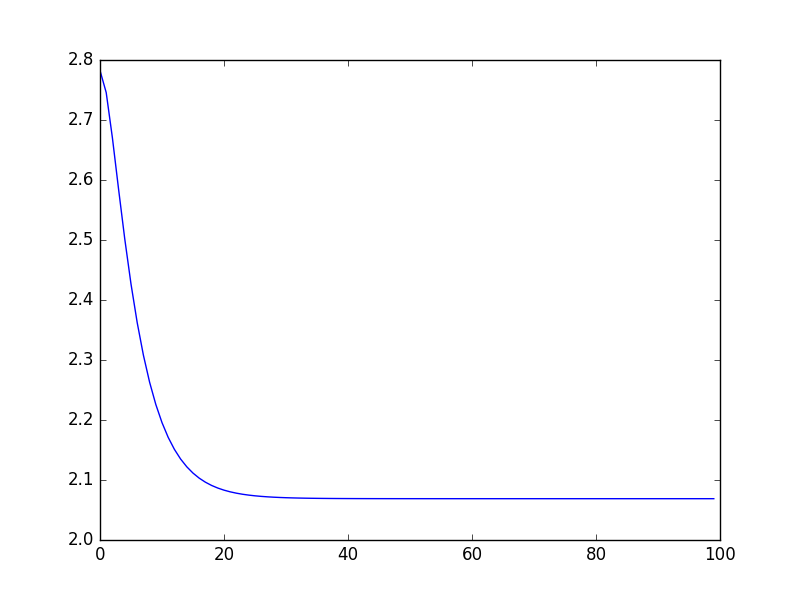
\includegraphics[width=\columnwidth]{figure/energy_has_lambda.png}
\caption{The energy converges to 2.08 with Goldstein ADMM}
\label{fig:energySame}
\end{figure}

\begin{figure}
\centering
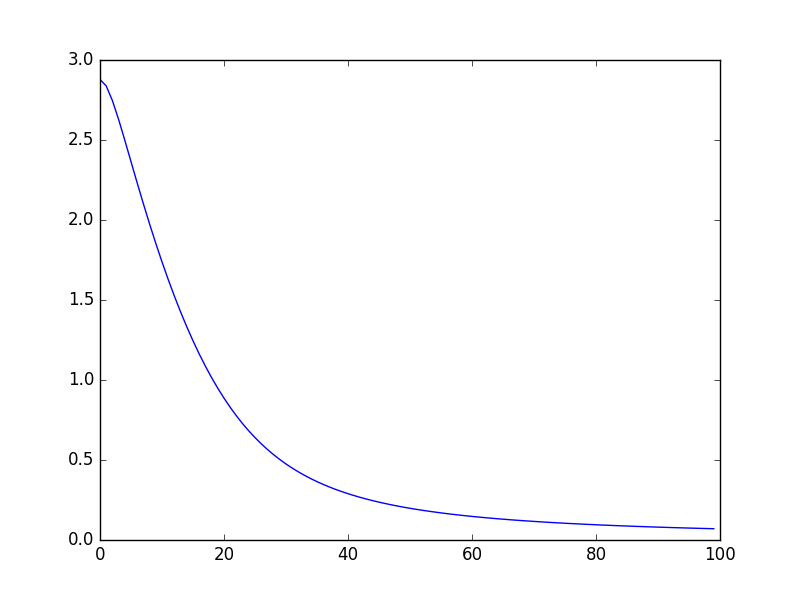
\includegraphics[width=\columnwidth]{figure/energy_no_lambda.png}
\caption{The energy converges to 0 without $\lambda$}
\label{fig:energyWithoutLambda}
\end{figure}

Recall the difference between the Goldstein ADMM and the classical ADMM, the Lagrange multiplier and the Bregman iteration might contribute to the low performance. Therefore, we remove the Lagrange item and only include the quadratic penalties into objective function.

We apply Algorithm \ref{alg:goldADMM} with $\lambda=0$ and deleting line 10 to solve equation \eqref{eq:quadratic_only}. A result with lower energy and higher accuracy is achieved, which is illustrated in Fig.\ref{fig:energyWithoutLambda}. Based on this fact, we guess the Bregman iteration and the Lagrange multiplier are the main reason for the low performance.

To analyze the reason mathematically, we introduce a simple problem:
\begin{equation}
\begin{aligned}
& \underset{w,a}{\text{minimize}}  & & (a-1)^2 \\
& \text{s.t.} & & w+a =2\\
\end{aligned}
\label{eq:demo}
\end{equation}
which can be viewed as an ANN with 1 layers and the dimension of $a$ is $\mathbb{R}$. Since the Bregman iteration is applied for linear problems, we simplify $w \cdot a$ with $w + a$. Applying the idea of equation \eqref{eq:breg_model}:
\begin{equation}
\begin{aligned}
& \underset{w,a}{\text{minimize}}  & & (a-1)^2 + \lambda \cdot a + \beta (2-w-a)^2\\
\end{aligned}
\end{equation}
Above problem can be solve by using the same procedure from \ref{alg:goldADMM}, at each iteration $k$, we can get
\begin{equation}
\begin{aligned}
w^{k+1} &= 2-a^k \\
a^{k+1} &= \frac{\lambda^k+2+4\beta-2\beta w^{k+1}}{2+2\beta}\\
\lambda^{k+1} &= \lambda^{k+1} + 2\beta(2-w^{k+1}-a^{k+1})\\
\end{aligned}
\label{eq:demoupdate}
\end{equation}
This test example cannot return the result $w=1,a=1$ unless one of them is initialized as 1. However, the result can always satisfy the constraint. This is because of the property of Bregman iteration: once a feasible result is achieved, the iteration stops and it is the optimal one. It is obvious that when $w^k$ and $a^k$ satisfy the constraints, equation \eqref{eq:demoupdate} will stop updating. To show the rest of this property, recall that Bregman iteration wants to minimize the Bregman distance $D^p_J(u,v) = J(u)-J(v)-<p,u-v>, p \in \partial J(v)$ which is nonnegative. Therefore, substitute our problem into the nonnegative inequality, for any $a$, we can get
\begin{equation}
\begin{aligned}
J(a^k) & \leq J(a) -(a-a^k) \cdot \lambda^k \\
& = J(a) - (a-(2-w^k)) \cdot \lambda^k \\
\end{aligned}
\end{equation}
which means for any $a$ that satisfies $a+w^k=2$, we can get the optimal $J(a)$. However, we cannot ensure that this $w^k$ is the optimal value, i.e. if the final $w^k$ is not optimal, the corresponding $a$ is not optimal.

In fact, we can construct a new value $u = [w,a]^T$ and rewrite the problem in equation \eqref{eq:demo}
\begin{equation}
\begin{aligned}
& \underset{u}{\text{minimize}}  & & ([0,1]\cdot u-1)^2 \\
& \text{s.t.} & & [1,1] \cdot u = 2\\
\end{aligned}
\end{equation}
then if we apply Bregman iteration to above problem, which is classical Bregman iteration, the result is correct. In this case, the Lagrange multiplier $\lambda$ is a 2x1 matrix, which means updating $w$ should consider $\lambda$.

All above are discussed in linear case, we also tested the same idea in nonlinear case, this Bregman iteration cannot work neither. Therefore, we conclude that the reason why Goldstein ADMM cannot work is that the Bregman iteration and Lagrange multiplier should not only be considered for $z_L$ only.

\section{Improvement based on Goldstein ADMM} \label{improvement}
In this section, we propose our improvement based on Goldstein ADMM. We first try to solve equation \eqref{eq:model} using classical ADMM. It turns out that classical ADMM cannot perform stably. Inspired by the quadratic penalty method, we include only $l_2$ norm penalty in to objective function. This method can return a sequence with decaying energy to 0. Nonetheless, the constraints in equation \eqref{eq:model} are satisfied slowly and even not satisfied if the parameter $\gamma, \beta$ are not chose correctly. Additionally, we notice that if $\beta$ in Algorithm \ref{alg:goldADMM} is sufficient small, it is almost same as the quadratic penalty method. Therefore, we figure out one algorithm which can converge to optimal solution to a certain degree and the constraints are satisfied.

\subsection{Quadratic penalty method}
According to previous analysis, the Lagrange multiplier and Bregman iteration are the causes why Algorithm \ref{alg:goldADMM} fails. Thus, we manage to solve the equation \eqref{eq:model} by using quadratic penalty method, which leads to the equation:
\begin{equation}
\begin{aligned}
\underset{\{W_l\},\{a_l\}, \{z_l\}}{\text{minimize}} 
& l(z_L,y) + \beta_L||z_L -W_La_{L-1}||^2 \\
+ \sum_{l=1}^{L-1}&[\gamma_l||a_l - h_l(z_l)||^2 + \beta_l||z_l - W_la_{l_1}||^2]
\label{eq:quadratic_only}
\end{aligned}
\end{equation}
This optimization problem can be solved by Algorithm \ref{alg:goldADMM} with a little modification mentioned before.

\begin{figure*}
\centering
\begin{subfigure}{0.8\columnwidth}
\centering
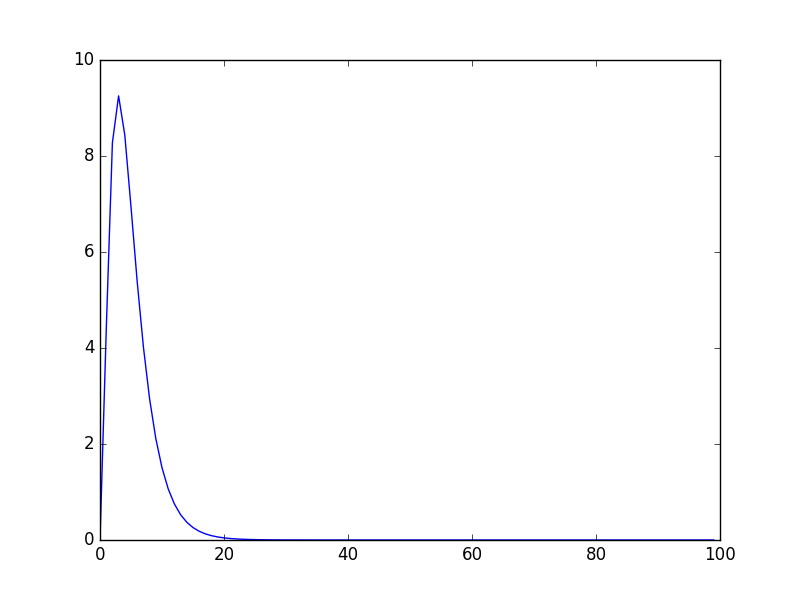
\includegraphics[width=0.7\columnwidth]{figure/aConstraint_has_lambda.png}
\caption{$||a_l-h_l(z_l)||^2$ with Lagrange multiplier $\lambda$}
\end{subfigure}
\begin{subfigure}{0.8\columnwidth}
\centering
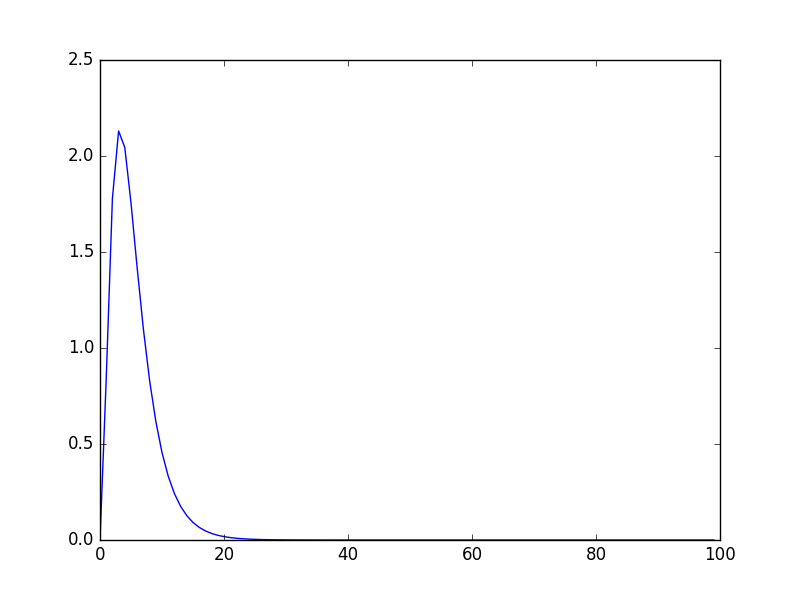
\includegraphics[width=0.7\columnwidth]{figure/zConstraint_has_lambda.png}
\caption{$||z_l-W_la_{l-1}||^2$ with Lagrange multiplier $\lambda$}
\end{subfigure}
\begin{subfigure}{0.8\columnwidth}
\centering
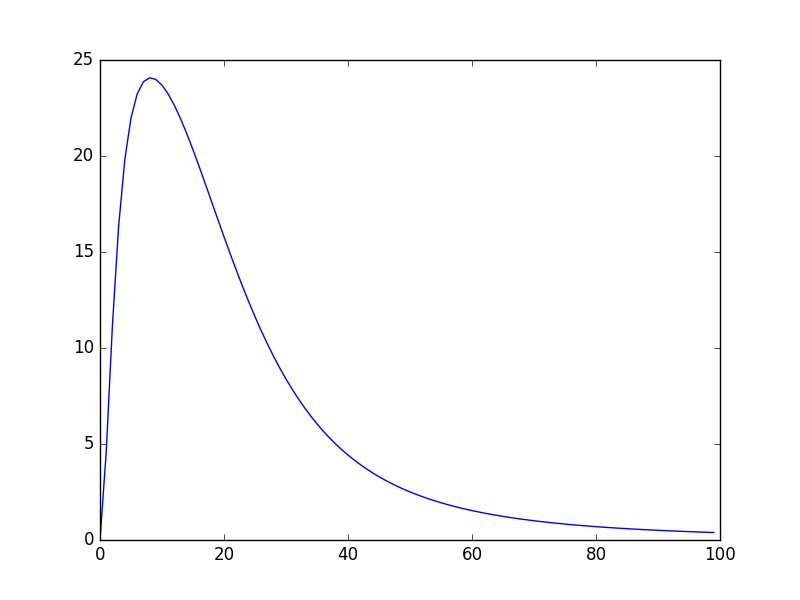
\includegraphics[width=0.7\columnwidth]{figure/aConstraint_no_lambda.png}
\caption{$||a_l-h_l(z_l)||^2$ without Lagrange multiplier $\lambda$}
\end{subfigure}
\begin{subfigure}{0.8\columnwidth}
\centering
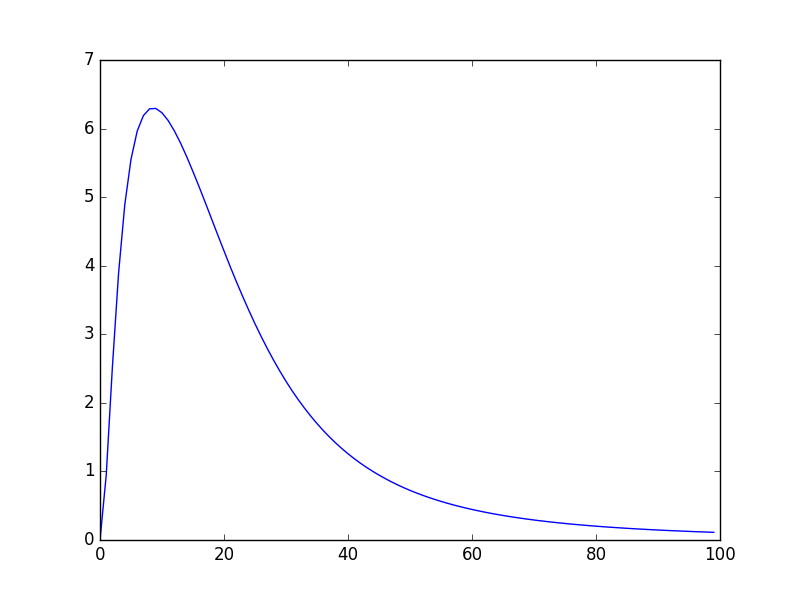
\includegraphics[width=0.7\columnwidth]{figure/zConstraint_no_lambda.png}
\caption{$||z_l-W_la_{l-1}||^2$ without Lagrange multiplier $\lambda$}
\end{subfigure}
\caption{The norm of constraints, $l=1$}
\label{fig:cmpCons}
\end{figure*}

It is obvious that once the optimal value is got, the corresponding $\{W_l\}$, $\{a_l\}$,$\{z_l\}$ are feasible for equation \eqref{eq:model}. However, the experiments show that the norms of constraints decays slowly, as illustrated in Fig.\ref{fig:cmpCons}. This is caused by the property of ADMM that original complex problem is decomposed into several simpler subproblems. Updating $\{a_l\}$ and $\{z_l\}$ become a trade-off between satisfying the constraints and minimizing loss function. If increasing the weight of each constraint, constraints are satisfied faster with higher loss energy. Additionally, increasing the iteration number can satisfy the constraints and lower the loss energy at the same time, which accounts for more computational expensive especially for large data set.

\begin{table*}[h]
\centering
\caption{Parameters and Results on MNIST}
\begin{tabular}{|c|c|c|c|c|c|c|c|c|c|}
\hline
	Hidden Layers & $\{\beta_l\}$ & $\{\gamma_l\}$ & $\rho$ & inIteration & outIteration & time & final energy & train accuracy & test accuracy\\
\hline
		(300) & 1e-6 & 1e-6 & 1.05 & 4 & 400 & 220s& 0.15378 & 95.4\% & 94.8\% \\
		(500,300) & 1e-8 & 1e-8 & 1.05 & 4 & 400 & 504s & 0.15871 & 95.2 \% & 95.1\% \\ 
\hline
\end{tabular}
\label{tab:parMNIST}
\end{table*}

\begin{table*}[h]
\centering
\caption{Parameters and Results on CrescentMoon}
\begin{tabular}{|c|c|c|c|c|c|c|c|c|c|}
\hline
	Hidden Layers & $\{\beta_l\}$ & $\{\gamma_l\}$ & $\rho$ & iters & time & final energy & train acc & test acc\\
\hline
		(50,50) & 1e-2 & 1e-2 & 1.01 & 450 &  71s & 0.1026 & 95.40\% & 94.74\% \\
		(10,10,10,10,10) & 1e-2 & 1e-2 & 1.02 & 450 & 18s & 0.1063 & 95.46 \% & 94.80\% \\ 
\hline
\end{tabular}
\label{tab:parMoon}
\end{table*}

\subsection{Bregman iteration with increasing penalty weights}
To overcome the disadvantage of quadratic penalty method, a time-saving algorithm, which can satisfy constraints and minimize loss function at the same time, is proposed. Inspired by above discussion about the weight of each constraints, in this algorithm, the penalty weights are increasing at each iteration. To improve the efficiency, we also implement mini-batch for this algorithm. Besides, the regularization item is involved in the object function to prevent over-fitting and numerical errors.

\begin{equation}
\begin{aligned} 
& \underset{\{W_l\},\{a_l\}, \{z_l\}}{\text{minimize}}
& & l(z_L,y) + \sum_{l=1}^L \alpha ||W_l||^2 \\
& \text{s.t.}
& & z_l = W_la_{l-1},  l = 1,2,...,L \\
& & & a_l = h_l(z_l),  l = 1,2,...L-1 \label{eq:modelWithReg}
\end{aligned}
\end{equation}
where $\alpha$ is the weight of regularization. The new algorithm to solve this optimization problem is described in Algorithm \ref{alg:ourADMM}.
\begin{algorithm} 
\caption{ADMM for Neural Networks}
\label{alg:ourADMM}
\KwIn{training features $\{a_0\}$, and labels $\{y\}$}
initialize $\{a_l\}^{L}_{l=1}$, $\{z_l\}^{L}_{l=1}$, $\lambda$ and weights\\
\For{i = 1, \dots, outIteration}{
	$a_0 \gets$ random batch\\
	\For {j = 1, \dots, inIteration}{
		\For{l = 1, 2, \dots, L-1}{
		 	$W_l \gets (\alpha+I)^{-1}z_la_{l-1}^T(I+a_{l-1}a_{l-1}^T)^{-1}$ \\
		 	$a_l \gets (\beta_{l+1}W_{l+1}^TW_{l+1}+\gamma_lI)^{-1}$\\  
	    		$~~~~~~ \cdot (\beta_{l+1}W_{l+1}^Tz_{l+1}+\gamma_lh_l(z_l))$\\
	    		$z_l \gets argmin_z ||a_l-h_l(z)||^2 + \beta_l||z-W_la_{l-1}||^2$\\
	    		$\beta_l \gets \beta_l \cdot \rho $
		}
		$W_L \gets (\alpha+I)^{-1}z_La_{L-1}^T(I+a_{L-1}a_{L-1}^T)^{-1}$\\
		$z_L \gets argmin_z \mathcal{L}(z,y)$\\
		$ ~~~~~~+ <z, \lambda> + \beta_L||z-W_La_{L-1}||^2$\\
		$\lambda \gets \lambda + \beta_L(z_L-W_La_{L-1})$\\
		$\beta_L \gets \beta_L \cdot \rho$\\
	}
}

\end{algorithm}

\textbf{Increasing penalty weights}: according to the discussion in quadratic penalty method, the weights of penalty play an important role in satisfying constraints and minimizing loss function. Therefore, the main idea is that the initial value of the weights are sufficient small and at each iteration, the weights are multiplied by a constant $\rho>1$. We also involve the Lagrange multiplier $\lambda$ and apply the same Bregman iteration as Goldstein ADMM to force the constraints to be satisfied faster. The main reason is that with small $\{beta_L\}$, the $\lambda$ has ignorable effect on updating $z_L$ since $\lambda$ is initialized with 0. Thus, at the beginning iterations, a $z_L$ which can minimizing the loss function sufficiently, is achieved. When the $\{beta_L\}$ becomes large enough, $z_L$ has to satisfy the constraints as well. To validate our idea, we still use equation \eqref{eq:demo}. $\beta$ is initialized with 0.0001 and $rho$ is 1.01. For each iteration $k$, we get
\begin{equation}
\begin{aligned}
w^{k+1} &= 2-a^k \\
a^{k+1} &= \frac{\lambda^k+2+4\beta-2\beta w^{k+1}}{2+2\beta}\\
\lambda^{k+1} &= \lambda^{k+1} + 2\beta(2-w^{k+1}-a^{k+1})\\
\beta &= \beta \cdot \rho \\
\end{aligned}
\label{eq:demoupdate}
\end{equation}
The test result is $x=1.0001, w=0.9999$. Even if the iteration number is increased, it cannot converge to the optimal result, which means this algorithm can only converges to the neighborhood of the optimal result. The radius of the neighborhood depends on the initial value of $\beta$. If $\beta$ is initialized with smaller positive value, a final result which is closer to optimal one is achieved, which coincides with above analysis. Another parameter $\rho$ is determined based on the initial value of $\beta$. Small $\rho$ leads to a slow speed of satisfying the constraints. Too large $\rho$ results in a high loss energy. Besides, this algorithm is also tested on nonlinear case and can work as well. Therefore, even with the disadvantage that it can only reach the neighborhood, we decide to apply this algorithm to solve equation \eqref{eq:model}.



\textbf{Other improvement}: We implement the mini-batch to our algorithm. The basic idea is that a batch is randomly chose from the data set. Then the neural network is trained by this batch. After several iterations, a new batch is chose and train the neural network based on previous results. Besides, we also include the regularization item for $\{W_l\}$ to solve the numerical errors and over-fitting. The new problem then becomes:


\section{Experiments} \label{experiment}
In this section, we show the numeric results of Alg \ref{alg:ourADMM} on three different datasets: Mnist and CresentMoon. The following experiments were run on CPU (MacBook Air Early 2014 with 1,7 GHz Intel Core i7). For every case, we pick weight decay as 1e-3.

\subsection{Mnist}
The Mnist dataset has 60,000 training images and 10000 tesing images. We used all 60,000 examples for training and didn't have any validation examples. To validate the algorithm, we trained the network with two structure and the corresponding result is shown in table  \ref{tab:parMNIST}.  In both case, we initialize the all weight matrices $w_l$ as zero mean Gaussian random weights with standard deviation $\epsilon$ = 1e-1.We applied mini-batch for training both of them for time efficiency. Each batch has 400 images, and 4 ADMM steps are applied per batch. We found that both networks are better trained by starting with very small penalty parameters $\{\beta_l\}$, $\{\gamma_l\}$ and then increasing them with small growing step $\rho$. Additionally, the same networks are trained without mini batch. The accuracy around 97\% and energy lower than 0.1 can be achieved, while the computational time becomes extremely long.

\subsection{CrescentMoon}
This dataset is much smaller than Mnist, with 6867 training images, no validation images and 3133 testing image. This time we didn't use mini-batch during training. Two different network structures are trained and the corresponding result is shown in table  \ref{tab:parMoon}. In both case, we initialize the all weight matrices $w_l$ as zero mean Gaussian random weights with standard deviation $\epsilon$ = 1e-2. For the second case with more hidden layers i.e. (10,10,10,10,10), we notice much more unstable performance of the Alg \ref{alg:ourADMM}, compared with the first case. In table \ref{tab:parMoon}, the first configuration we can always get accuracy around 95.4\%. However, with the second configuration, the algorithm sometimes give testing accuracy only around 80\%, even though one can get accuracy around 95.4\% after several tryings.  In addition, we found for case two several settings can reach close testing accuracy, but also has similar unstable behavior. The reason of such an instability is not clear to us yet.

\section{Conclusion} \label{conclusion}
We implemented the ADMM from Goldstein on MNIST data set. However, this ADMM fails to achieve an expected result, which is caused by the Bregman iteration according to our analysis on a simple optimizing problem. To improve the Goldstein ADMM, we propose the ADMM with increasing weight parameters for constraints and the Bregman iteration is still applied to our ADMM. The experiement results show that this ADMM can achieve a higher accuracy and lower energy. There are still some open questions about this ADMM: i) the algorithm can only converge to the neighborhood of optimal results; ii) the instability for different data set; iii) the converge analysis of this ADMM.

\balance
%\addtolength{\textheight}{-10cm}   % This command serves to balance the column lengths
                                  % on the last page of the document manually. It shortens
                                  % the textheight of the last page by a suitable amount.
                                  % This command does not take effect until the next page
                                  % so it should come on the page before the last. Make
                                  % sure that you do not shorten the textheight too much.

%%%%%%%%%%%%%%%%%%%%%%%%%%%%%%%%%%%%%%%%%%%%%%%%%%%%%%%%%%%%%%%%%%%%%%%%%%%%%%%%

\begin{thebibliography}{99}

\bibitem{1} "The Machine Learning Dictionary" , \url{http://www.cse.unsw.edu.au/~billw/mldict.html}

\bibitem{2} Dean, Jeffrey, et al. "Large scale distributed deep networks." Advances in neural information processing systems. 2012.


\bibitem{3} Choromanska, Anna, et al. "The Loss Surfaces of Multilayer Networks." AISTATS. 2015.

\bibitem{4} Dauphin, Yann N., et al. "Identifying and attacking the saddle point problem in high-dimensional non-convex optimization." Advances in neural information processing systems. 2014.

\bibitem{5} Xu, Zheng, et al. "An empirical study of admm for nonconvex problems." arXiv preprint arXiv:1612.03349 (2016).

\bibitem{6} Hong, Mingyi, Zhi-Quan Luo, and Meisam Razaviyayn. "Convergence analysis of alternating direction method of multipliers for a family of nonconvex problems." SIAM Journal on Optimization 26.1 (2016): 337-364.

\bibitem{7} Wang, Yu, Wotao Yin, and Jinshan Zeng. "Global convergence of ADMM in nonconvex nonsmooth optimization." arXiv preprint arXiv:1511.06324 (2015).

\bibitem{8} Wang, Fenghui, Zongben Xu, and Hong-Kun Xu. "Convergence of Bregman alternating direction method with multipliers for nonconvex composite problems." arXiv preprint arXiv:1410.8625 (2014).

\bibitem{9} Taylor, Gavin, et al. "Training neural networks without gradients: A scalable admm approach." International Conference on Machine Learning. 2016.

\bibitem{10} Goldstein, Tom, and Stanley Osher. "The split Bregman method for L1-regularized problems." SIAM journal on imaging sciences 2.2 (2009): 323-343.





\end{thebibliography}
\end{document}
